\documentclass[11pt,a4paper]{article}
\usepackage[margin=0.9in]{geometry}
\usepackage{amsmath,amssymb,amsthm}
\usepackage{booktabs,longtable,array,multirow}
\usepackage{graphicx,float,subcaption}
\usepackage{xcolor}
\usepackage{enumitem}
\usepackage{hyperref}
\usepackage[numbers]{natbib}
\usepackage{tikz}
\usetikzlibrary{arrows.meta,positioning,fit,calc,shapes.geometric,backgrounds}
\usepackage{pgfplots}
\pgfplotsset{compat=1.18}
\usepackage{caption}
\usepackage{microtype}
\hypersetup{colorlinks=true,linkcolor=blue!60!black,citecolor=blue!60!black,urlcolor=blue!60!black}
\setlength{\parskip}{0.42em}
\setlength{\parindent}{0pt}
\renewcommand{\arraystretch}{1.12}
\newcommand{\R}{\mathbb{R}}
\newcommand{\one}{\mathbf{1}}
\definecolor{nyuviolet}{RGB}{87,6,140}
\definecolor{deepblue}{RGB}{35,65,120}
\tikzset{block/.style={rectangle, rounded corners=3pt, draw=nyuviolet!70, very thick, fill=nyuviolet!6, align=center, minimum height=0.88cm, text width=3.2cm}, smallblock/.style={rectangle, rounded corners=2pt, draw=deepblue!65, thick, fill=deepblue!5, align=center, minimum height=0.68cm, text width=2.8cm}, arrow/.style={-{Latex[length=2.5mm]}, thick, draw=black!65}, heatcell/.style={rectangle, minimum width=3.25cm, minimum height=0.72cm, draw=white, line width=1.0pt, font=\small\bfseries, align=center}}

\title{\textbf{Context-Aware Portfolio Allocation as Layered System Optimization:}\\ Universe Breadth, Screening, Controller Choice, and Learned Routing}
\author{Ashesh Kaji\\ \textit{System Optimization Methods, New York University}\\ \href{mailto:ask9184@nyu.edu}{ask9184@nyu.edu}}
\date{April 2026}
\begin{document}
\maketitle

\begin{abstract}
This paper studies portfolio allocation as a layered system optimization problem rather than as a single static mean--variance solve. The central thesis is that a practical allocation system contains several control layers: the parent universe, the screening or cardinality rule, the within-screen weighting controller, and a higher-level model-selection or routing policy. The empirical study extends an initial comparison of model-based and reinforcement-learning controllers into a mechanism-identification experiment over liquid U.S. equity candidate universes of different breadth. A screen-integrated walk-forward matrix evaluates 60 universe--screen--controller arms at a canonical 10 basis point transaction-cost slice, while retaining split-level ledgers, cost sensitivity, turnover, multiple-comparison diagnostics, and an integrated reinforcement-learning routing study. The main empirical result is that the preferred control stack changes with universe breadth: a 21-day momentum screen followed by equal weighting is strongest in the top-100 candidate universe, a low-volatility screen followed by equal weighting is strongest in the top-250 candidate universe, and a volatility-adjusted momentum screen followed by a 21-day rank-and-hold controller is strongest in the top-500 candidate universe. A policy-gradient router over the same screened-control arms learns stable, economically interpretable selections and improves over train-selected fixed selection in the combined panel, but it does not dominate a simple trailing-window router. The practical conclusion is deliberately layered: portfolio performance should be improved first by matching universe construction, screening, and weighting mechanics to the opportunity set, and only then by adding learned routing on top of a well-characterized action set.
\end{abstract}

\section{Introduction}
Portfolio optimization is often introduced as a one-shot decision: estimate expected returns $\mu$ and covariances $\Sigma$, then choose weights $w$ on the simplex by solving
\begin{equation}
\max_{w \in \R^n} \quad \mu^{\top}w - \lambda w^{\top}\Sigma w
\quad\text{s.t.}\quad \one^{\top}w=1,\; w\geq 0.
\label{eq:markowitz}
\end{equation}
This view is foundational, but incomplete for an operational allocation problem. A live portfolio system repeatedly chooses which securities are eligible, which features define the active opportunity set, how concentrated the portfolio should be, how much turnover is tolerable, and whether recent evidence should change the controller itself. The optimization problem is therefore not one decision but a hierarchy of decisions.

The motivating question for this study is: \emph{Can practical portfolio performance be improved by treating allocation as a layered control problem in which universe breadth, screening, weighting, and routing are studied jointly rather than independently?}

The first phase of the project compared broad controller families: momentum rank-and-hold, mean-reversion scoring, convex mean--variance with turnover, regime-adaptive composites, online signal weighting, and policy-gradient allocation. That phase established the baseline system-optimization perspective: controller identity matters, transaction costs matter, and the best controller depends on the statistical structure of the asset universe. The present paper pushes the research deeper. Instead of only asking which weighting rule is best, it asks which \emph{control stack} is best: candidate universe breadth $\rightarrow$ screen/cardinality rule $\rightarrow$ weighting controller $\rightarrow$ optional learned router.

\section{Research Questions and Contributions}
The study is organized around four questions.
\begin{enumerate}[leftmargin=1.5em]
    \item \textbf{Universe-breadth dependence.} Does the preferred portfolio controller change when the candidate universe expands from roughly 100 liquid equities to 250 and 500 candidates?
    \item \textbf{Screening as a control layer.} Is screening merely preprocessing, or does it independently change the best risk-adjusted outcome?
    \item \textbf{Weighting after screening.} Once a screen has selected a compact holding set, is a more active rank-and-hold controller still better than equal weighting?
    \item \textbf{Learned meta-control.} Can a learned router over screen/controller arms improve over deployable fixed or trailing-window selection rules?
\end{enumerate}
The contributions are correspondingly fourfold. First, the paper formulates portfolio construction as a layered control system. Second, it evaluates a screen-integrated walk-forward matrix with explicit transaction costs and provenance ledgers. Third, it reports mechanism-level ablations over screen and controller layers rather than only winner tables. Fourth, it integrates reinforcement learning as a meta-control layer over already-defined portfolio arms, with repeated seeds and explicit baselines rather than a single anecdotal training curve.

\section{Related Work}
The baseline optimization language comes from Markowitz's mean--variance framework \citep{markowitz1952portfolio}. Dynamic trading with predictable returns and transaction costs motivates the view that turnover is a control cost and that optimal policies should partially adjust rather than rebalance without friction \citep{garleanu2013dynamic}. Empirical evidence that naive diversification can be difficult to beat out of sample also motivates treating equal weight as a serious baseline rather than a straw man \citep{demiguel2009optimal}. Universal portfolio and online expert methods show that allocation can be viewed as sequential learning across competing rules \citep{cover1991universal}. Reinforcement learning adds a model-free sequential-decision lens, but financial RL is sensitive to environment design, state representation, and evaluation protocol \citep{williams1992simple,jiang2017deep,zhang2020deep}. Finally, multiple-testing concerns in strategy research require explicit discipline when many alternatives are evaluated \citep{bailey2014deflated}.

\section{Layered Control Formulation}
Let $\mathcal{U}_b(t)$ denote a candidate universe at breadth level $b \in \{100,250,500\}$, and let $S_j$ denote a screening rule that maps historical prices through date $t$ into a holding set $H_{b,j}(t) \subset \mathcal{U}_b(t)$. A weighting controller $C_k$ maps the screened price history and current portfolio state into target weights. The portfolio decision can be written as
\begin{equation}
w_t = C_k\big(S_j(\mathcal{U}_b, \mathcal{F}_t),\; \mathcal{F}_t,\; w_{t^-}\big),
\label{eq:composition}
\end{equation}
where $\mathcal{F}_t$ is the information available at rebalance time and $w_{t^-}$ is the pre-trade portfolio. A higher-level router selects the tuple $(b,j,k)$ or, within a fixed universe scope, the arm $(j,k)$.

\begin{figure}[H]
\centering
\resizebox{0.98\textwidth}{!}{%
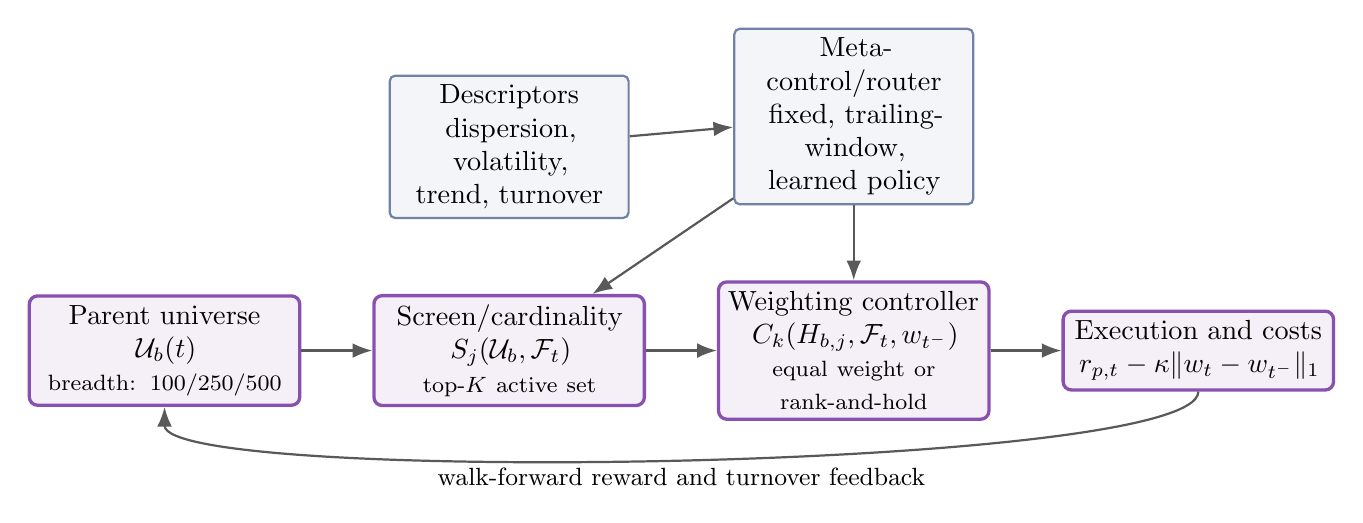
\begin{tikzpicture}[node distance=0.7cm and 0.9cm]
\node[block] (universe) {Parent universe\\$\mathcal{U}_b(t)$\\\footnotesize breadth: 100/250/500};
\node[block, right=of universe] (screen) {Screen/cardinality\\$S_j(\mathcal{U}_b,\mathcal{F}_t)$\\\footnotesize top-$K$ active set};
\node[block, right=of screen] (weight) {Weighting controller\\$C_k(H_{b,j},\mathcal{F}_t,w_{t^-})$\\\footnotesize equal weight or rank-and-hold};
\node[block, right=of weight] (execution) {Execution and costs\\$r_{p,t}-\kappa\|w_t-w_{t^-}\|_1$};
\node[smallblock, above=0.95cm of screen] (desc) {Descriptors\\dispersion, volatility, trend, turnover};
\node[smallblock, above=0.95cm of weight] (router) {Meta-control/router\\fixed, trailing-window, learned policy};
\draw[arrow] (universe) -- (screen);
\draw[arrow] (screen) -- (weight);
\draw[arrow] (weight) -- (execution);
\draw[arrow] (desc) -- (router);
\draw[arrow] (router) -- (screen);
\draw[arrow] (router) -- (weight);
\draw[arrow] (execution.south) .. controls +(0,-1.0) and +(0,-1.0) .. node[below, font=\small] {walk-forward reward and turnover feedback} (universe.south);
\end{tikzpicture}}
\caption{Layered portfolio-control architecture used in the empirical study. The experiment separates universe construction, screening, weighting, and routing so performance can be attributed to mechanisms rather than to a monolithic strategy label.}
\label{fig:layered_architecture}
\end{figure}

The screen rules are simple and interpretable:
\begin{align}
\text{Momentum}_{i,\tau}(t) &= P_i(t)/P_i(t-\tau)-1,\\
\text{VolAdjMom}_{i,\tau}(t) &= \frac{P_i(t)/P_i(t-\tau)-1}{\widehat{\sigma}_{i,\tau}(t)+\epsilon},\\
\text{LowVol}_{i,\tau}(t) &= -\widehat{\sigma}_{i,\tau}(t).
\end{align}
The cluster-capped momentum screen first groups highly correlated assets and then limits the number of selected names per group, reducing the chance that the top-$K$ list is dominated by near-duplicate exposures. Equal weighting assigns $w_i=1/|H|$ for $i\in H$. Rank-and-hold controllers compute lookback returns over $\tau\in\{21,63,126\}$ days and hold the top five names in the screened set. Net return includes transaction costs:
\begin{equation}
R_{p,t}^{\text{net}} = w_t^\top r_{t+1} - \kappa \|w_t-w_{t^-}\|_1.
\end{equation}
The canonical reported cost is $\kappa=10$ basis points, with 0 and 25 basis point slices retained for robustness diagnostics.

\section{Experimental Design}
The context-aware experiment uses three liquid U.S. equity candidate-universe breadth levels. The top-100, top-250, and top-500 labels describe parent candidate breadths, while the implemented pilots use symbol limits of 25, 40, and 60 respectively for tractable walk-forward execution. This limitation is explicit because the current universe lists are current-constituent based and therefore survivorship-biased rather than point-in-time membership files.

Each experiment is evaluated through chronology-respecting walk-forward splits. Screens are computed using data available through the training end date, and evaluation metrics are measured on the subsequent test interval. The final screen-integrated core matrix evaluates five screens and four controllers across three universe scopes, for 60 canonical arms at the 10 basis point cost slice.

The experiment records provenance and selection information in machine-readable artifacts. The universe-provenance ledger identifies current-constituent and delisted-name limitations. The model-selection ledger records all tried configurations, not only winners. The split-level all-trials file preserves fold-level returns, drawdowns, and turnover so later robustness checks can be performed without rerunning the study.

\section{Main Results: Universe--Screen--Controller Matrix}
Table~\ref{tab:winners} gives the cleanest summary of the core result. The winning stack changes as the candidate universe broadens.
\begin{table}[H]
\centering
\caption{Best screen/controller stack by candidate-universe breadth. Metrics are mean walk-forward values at the 10 basis point transaction-cost slice.}
\label{tab:winners}
\small
\resizebox{\textwidth}{!}{%
\begin{tabular}{lllrrrrr}
\toprule
Universe & Screen & Controller & Splits & Ann. ret. & Ann. vol. & Sharpe & Worst DD \\
\midrule
Top-100 liquid equities & 21-day momentum, top 10 & Equal weight & 22 & 20.4\% & 20.2\% & 1.474 & -44.9\% \\
Top-250 liquid equities & 63-day low volatility, top 10 & Equal weight & 11 & 11.2\% & 14.1\% & 0.859 & -10.5\% \\
Top-500 liquid equities & Vol.-adjusted 63-day momentum, top 10 & 21-day rank-and-hold & 9 & 35.1\% & 20.8\% & 1.756 & -15.5\% \\
\bottomrule
\end{tabular}%
}
\end{table}

The top-100 result suggests that once a compact momentum-selected opportunity set is formed, equal weighting is difficult to beat. The top-250 result shifts toward low-volatility screening, indicating that risk filtering can dominate when the middle-breadth universe does not produce clean enough cross-sectional momentum dispersion. The top-500 result is the strongest evidence for the breadth thesis: with a broader candidate set, volatility-adjusted momentum identifies a richer opportunity set, and an additional short-horizon rank-and-hold layer improves realized Sharpe.

\begin{figure}[H]
\centering
\resizebox{0.98\textwidth}{!}{%
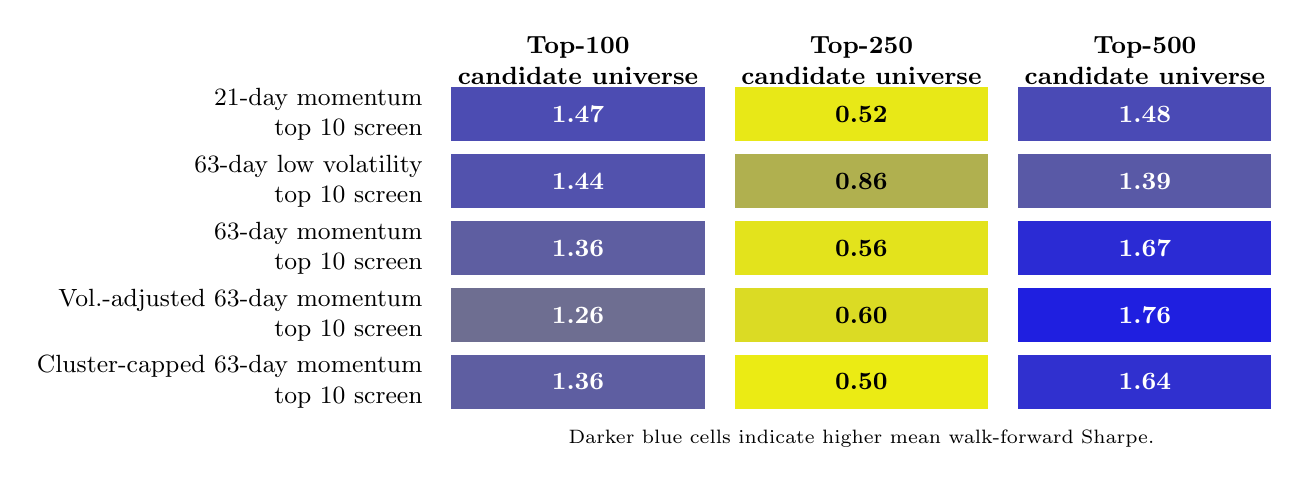
\begin{tikzpicture}
\node[heatcell, fill=blue!70!yellow, text=white] at (0.0,0.0) {1.47};
\node[heatcell, fill=blue!9!yellow, text=black] at (3.6,0.0) {0.52};
\node[heatcell, fill=blue!71!yellow, text=white] at (7.2,0.0) {1.48};
\node[heatcell, fill=blue!68!yellow, text=white] at (0.0,-0.85) {1.44};
\node[heatcell, fill=blue!31!yellow, text=black] at (3.6,-0.85) {0.86};
\node[heatcell, fill=blue!65!yellow, text=white] at (7.2,-0.85) {1.39};
\node[heatcell, fill=blue!63!yellow, text=white] at (0.0,-1.7) {1.36};
\node[heatcell, fill=blue!11!yellow, text=black] at (3.6,-1.7) {0.56};
\node[heatcell, fill=blue!83!yellow, text=white] at (7.2,-1.7) {1.67};
\node[heatcell, fill=blue!57!yellow, text=white] at (0.0,-2.55) {1.26};
\node[heatcell, fill=blue!14!yellow, text=black] at (3.6,-2.55) {0.60};
\node[heatcell, fill=blue!88!yellow, text=white] at (7.2,-2.55) {1.76};
\node[heatcell, fill=blue!63!yellow, text=white] at (0.0,-3.4) {1.36};
\node[heatcell, fill=blue!8!yellow, text=black] at (3.6,-3.4) {0.50};
\node[heatcell, fill=blue!81!yellow, text=white] at (7.2,-3.4) {1.64};
\foreach \j/\name in {0/{Top-100},1/{Top-250},2/{Top-500}} {\node[font=\small\bfseries, align=center] at (\j*3.6,0.68) {\name\\candidate universe};}
\foreach \i/\name in {0/{21-day momentum},1/{63-day low volatility},2/{63-day momentum},3/{Vol.-adjusted 63-day momentum},4/{Cluster-capped 63-day momentum}} {\node[font=\small, anchor=east, align=right] at (-1.85,-\i*0.85) {\name\\top 10 screen};}
\node[font=\scriptsize, align=center] at (3.6,-4.12) {Darker blue cells indicate higher mean walk-forward Sharpe.};
\end{tikzpicture}}
\caption{Best mean walk-forward Sharpe ratio by universe breadth and screen rule. Each cell chooses the best controller within that universe/screen pair. The broadest candidate set rewards volatility-adjusted and medium-horizon momentum screens, while the intermediate universe is persistently weaker.}
\label{fig:native_heatmap}
\end{figure}

\begin{figure}[H]
\centering
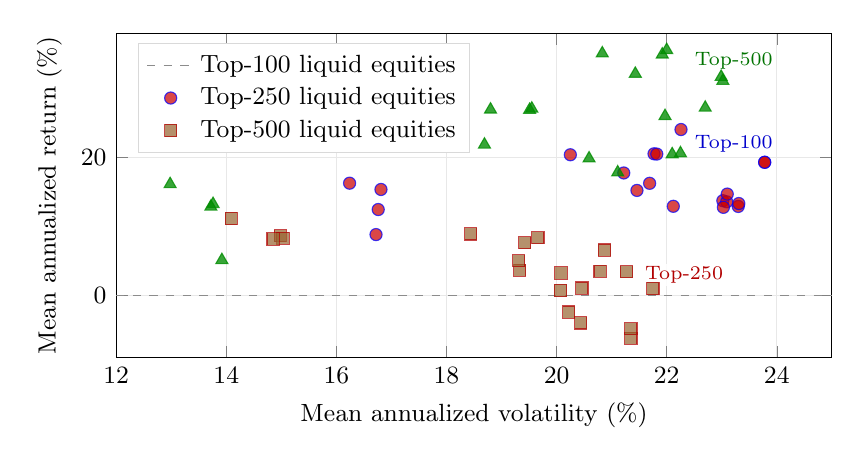
\begin{tikzpicture}
\begin{axis}[width=0.88\textwidth,height=0.47\textwidth,xlabel={Mean annualized volatility (\%)},ylabel={Mean annualized return (\%)},xmin=12,xmax=25,ymin=-9,ymax=38,grid=both,grid style={gray!18},legend pos=north west,legend style={font=\small, fill=white, draw=gray!30, cells={anchor=west}},tick label style={font=\small},label style={font=\small}]
\addplot[black!45, dashed, domain=12:25] {0};
\addplot+[only marks, mark=*, mark size=2.2pt, color=blue, opacity=0.72] coordinates {(21.77,20.55) (23.78,19.32) (23.02,13.75) (23.30,12.92) (16.24,16.29) (16.81,15.38) (16.76,12.47) (16.72,8.84) (20.25,20.41) (22.26,24.07) (21.69,16.27) (21.46,15.24) (21.82,20.51) (23.78,19.32) (23.09,13.59) (23.31,13.34) (21.22,17.77) (22.12,12.94) (23.10,14.71) (23.03,12.79)};
\addlegendentry{Top-100 liquid equities}
\addplot+[only marks, mark=square*, mark size=2.2pt, color=red!70!black, opacity=0.72] coordinates {(19.42,7.67) (20.79,3.51) (20.07,0.73) (21.35,-6.19) (14.09,11.18) (14.98,8.68) (15.03,8.31) (14.85,8.20) (20.87,6.59) (19.33,3.66) (21.75,1.01) (20.22,-2.39) (19.66,8.38) (21.27,3.46) (20.46,1.08) (21.35,-4.81) (18.44,8.93) (19.31,5.05) (20.08,3.27) (20.44,-3.97)};
\addlegendentry{Top-250 liquid equities}
\addplot+[only marks, mark=triangle*, mark size=2.5pt, color=green!55!black, opacity=0.78] coordinates {(21.92,34.94) (19.51,26.92) (22.99,31.70) (22.25,20.63) (12.98,16.15) (13.72,12.88) (13.76,13.27) (13.92,5.14) (21.43,32.15) (18.69,21.88) (21.97,26.02) (20.59,19.88) (22.00,35.59) (19.55,27.10) (23.02,31.12) (22.10,20.48) (20.83,35.11) (18.80,26.96) (22.70,27.23) (21.11,17.85)};
\addlegendentry{Top-500 liquid equities}
\node[anchor=west, font=\scriptsize, text=green!45!black, fill=white, fill opacity=0.85, text opacity=1, inner sep=1pt] at (axis cs:22.45,34.0) {Top-500};
\node[anchor=west, font=\scriptsize, text=red!70!black, fill=white, fill opacity=0.85, text opacity=1, inner sep=1pt] at (axis cs:21.55,3.0) {Top-250};
\node[anchor=west, font=\scriptsize, text=blue!80!black, fill=white, fill opacity=0.85, text opacity=1, inner sep=1pt] at (axis cs:22.45,22.0) {Top-100};
\end{axis}
\end{tikzpicture}
\caption{Risk--return map for the 60 screen/controller arms at the 10 basis point cost slice. Values are mean walk-forward annualized return and volatility. The green triangle cluster, corresponding to the top-500 candidate universe, contains the clearest favorable return region, while the red square cluster for the top-250 universe is persistently weaker at comparable volatility.}
\label{fig:risk_return_native}
\end{figure}

Because the study evaluates many arms, Table~\ref{tab:multiple_testing} reports the winner gap against the second-best arm within each universe. The small gap in the top-100 universe means the exact winner should not be overinterpreted; both low-volatility and 21-day momentum screens are competitive. The larger gaps in the top-250 and top-500 universes provide more useful mechanism evidence, although no formal p-values are claimed because folds overlap and arms are not independent.
\begin{table}[H]
\centering
\caption{Exploratory multiple-comparison diagnostic. The table reports the best and second-best mean Sharpe within each universe; it is not a formal significance test.}
\label{tab:multiple_testing}
\small
\begin{tabular}{p{2.7cm}rp{6.0cm}rrr}
\toprule
Universe & Arms & Best stack & Best SR & Second SR & Gap \\
\midrule
Top-100 & 20 & 21-day momentum, top 10 + Equal weight & 1.474 & 1.440 & 0.034 \\
Top-250 & 20 & 63-day low volatility, top 10 + Equal weight & 0.859 & 0.755 & 0.104 \\
Top-500 & 20 & Vol.-adjusted 63-day momentum, top 10 + 21-day rank-and-hold & 1.756 & 1.666 & 0.090 \\
\bottomrule
\end{tabular}
\end{table}

\section{Mechanism Interpretation}
The most useful practical findings are not only the winners, but the layer-specific lessons.
\paragraph{Screening is an actual control layer.} Averaging over controllers, the best screen changes with the universe. Low-volatility screening is strongest on average for the top-100 and top-250 scopes, while 63-day momentum is strongest on average for the top-500 scope. This means screening is not cosmetic preprocessing. It changes the feasible active set in a way that can dominate the subsequent weighting rule.
\paragraph{Equal weight remains a serious baseline after screening.} Equal weighting is the best average controller over screens in the top-100 and top-250 scopes. This is consistent with the empirical literature warning that estimation-heavy portfolio optimization can underperform simple diversification out of sample. In this experiment, once the screen has concentrated the opportunity set, a second high-turnover ranking layer often adds costs and instability without enough additional signal.
\paragraph{Breadth makes additional control useful.} The exception is the top-500 scope. There, the 21-day rank-and-hold controller has the best average Sharpe over screens, and the overall winner combines volatility-adjusted momentum screening with short-horizon ranking. The practical interpretation is that broad universes create more room for cross-sectional selection, but raw selection must be normalized by volatility to avoid simply buying noisy winners.
\paragraph{The top-250 result is a research warning.} The top-250 scope is consistently weaker across the heatmap and risk--return map. This may reflect the specific symbol-limited candidate construction, a less favorable middle-breadth opportunity set, or instability introduced by the filtering process. A strong final paper should not hide this result. It motivates a deeper follow-up using point-in-time membership and larger independent walk-forward samples.

\section{Integrated Reinforcement-Learning Routing Study}
The learned component is framed as a meta-controller, not as an unconstrained direct-weight allocator. For a fixed scope, define each screen/controller pair as an arm $a\in\mathcal{A}$. At decision time $t$, the router observes features containing time, scope identity where applicable, trailing arm rewards, and the most recent reward vector. It selects one arm and receives the next-period net reward minus a switching penalty. A policy-gradient procedure is evaluated against deployable and diagnostic baselines.

This design is important: the learned policy is not asked to rediscover portfolio construction from raw prices. It is asked a more appropriate system-optimization question: can a learned controller route among already interpretable control stacks better than simple model-selection rules?

\begin{table}[H]
\centering
\caption{Integrated reinforcement-learning router results. Rewards are cumulative test-period rewards at the canonical cost slice. RL values are mean $\pm$ standard deviation over seven seeds for the best policy-gradient configuration in each scope.}
\label{tab:rl_results}
\scriptsize
\begin{tabular}{p{2.15cm}rrrrrrrr}
\toprule
Scope & Test periods & RL & Train-fixed & Trailing & Random & Oracle & RL--fixed & RL--trailing \\
\midrule
Combined panel & 14 & 1.213 $\pm$ 0.063 & 1.134 & 1.543 & 1.276 & 2.586 & 0.079 & -0.330 \\
Top-100 liquid equities & 8 & 0.823 $\pm$ 0.011 & 0.827 & 0.475 & 0.657 & 1.355 & -0.004 & 0.348 \\
Top-250 liquid equities & 5 & 0.280 $\pm$ 0.068 & 0.305 & 0.306 & 0.296 & 0.764 & -0.026 & -0.026 \\
Top-500 liquid equities & 4 & 0.371 $\pm$ 0.000 & 0.371 & 0.566 & 0.525 & 0.932 & 0.000 & -0.196 \\
\bottomrule
\end{tabular}
\end{table}

\begin{figure}[H]
\centering
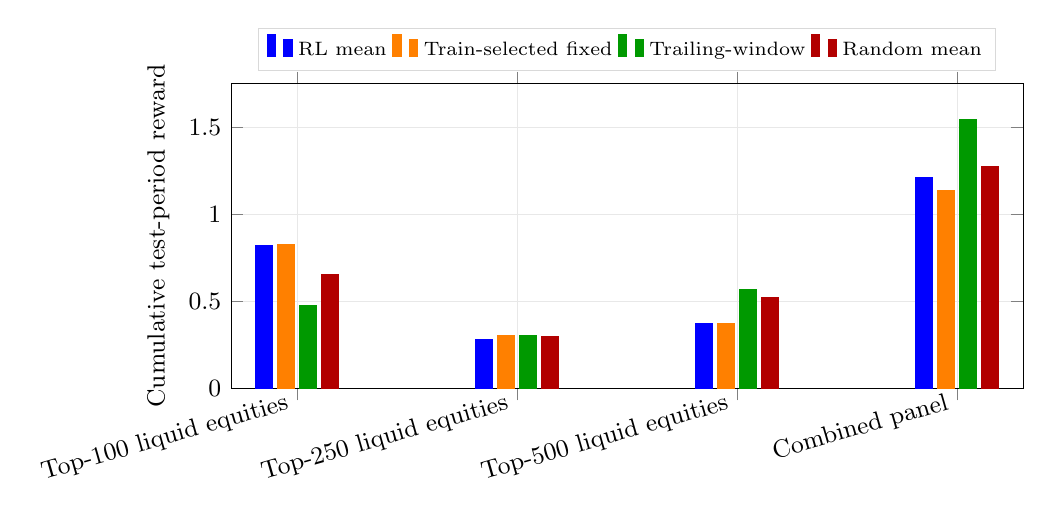
\begin{tikzpicture}
\begin{axis}[ybar,bar width=6pt,width=0.96\textwidth,height=0.45\textwidth,ylabel={Cumulative test-period reward},symbolic x coords={Top-100 liquid equities,Top-250 liquid equities,Top-500 liquid equities,Combined panel},xtick=data,x tick label style={rotate=16, anchor=east, font=\small},ymin=0,ymax=1.75,grid=major,grid style={gray!18},legend style={at={(0.5,1.04)}, anchor=south, legend columns=4, font=\scriptsize, draw=gray!30},tick label style={font=\small},label style={font=\small}]
\addplot+[ybar, fill=blue, draw=blue] coordinates {(Top-100 liquid equities,0.823) (Top-250 liquid equities,0.280) (Top-500 liquid equities,0.371) (Combined panel,1.213)};
\addlegendentry{RL mean}
\addplot+[ybar, fill=orange, draw=orange] coordinates {(Top-100 liquid equities,0.827) (Top-250 liquid equities,0.305) (Top-500 liquid equities,0.371) (Combined panel,1.134)};
\addlegendentry{Train-selected fixed}
\addplot+[ybar, fill=green!60!black, draw=green!60!black] coordinates {(Top-100 liquid equities,0.475) (Top-250 liquid equities,0.306) (Top-500 liquid equities,0.566) (Combined panel,1.543)};
\addlegendentry{Trailing-window}
\addplot+[ybar, fill=red!70!black, draw=red!70!black] coordinates {(Top-100 liquid equities,0.657) (Top-250 liquid equities,0.296) (Top-500 liquid equities,0.525) (Combined panel,1.276)};
\addlegendentry{Random mean}
\end{axis}
\end{tikzpicture}
\caption{Model-selection and routing baselines for the integrated learned-router study. The learned router is most useful relative to train-selected fixed selection in the combined panel, but trailing-window routing remains a strong non-RL benchmark in the combined and top-500 scopes.}
\label{fig:rl_native_bar}
\end{figure}

The learned router is still informative because its selected arms are stable and economically interpretable. Table~\ref{tab:rl_stability} reports seed-level win counts and dominant selections. The policy repeatedly selects momentum/rank-and-hold structures in the top-100 and top-500 scopes, and a low-volatility/equal-weight structure in the top-250 scope. These choices mirror the mechanism-level findings from the non-RL matrix.
\begin{table}[H]
\centering
\caption{Stability diagnostics for the best RL configuration. Each comparator column reports the number of random seeds, out of seven, in which the RL router outperforms the named comparator.}
\label{tab:rl_stability}
\scriptsize
\begin{tabular}{p{1.55cm}rrrp{6.55cm}}
\toprule
Scope & vs fixed & vs trailing & vs random & Dominant learned selection \\
\midrule
Combined panel & 6/7 & 0/7 & 1/7 & Cluster-capped 63-day momentum, top 10 + Equal weight \\
Top-100 & 6/7 & 7/7 & 7/7 & 21-day momentum, top 10 + 126-day rank-and-hold \\
Top-250 & 0/7 & 0/7 & 6/7 & 63-day low volatility, top 10 + Equal weight \\
Top-500 & 7/7 & 0/7 & 0/7 & 21-day momentum, top 10 + 63-day rank-and-hold \\
\bottomrule
\end{tabular}
\end{table}

The conclusion is nuanced. Reinforcement learning belongs in the main methodology because it tests the existence of a learnable routing layer. But the current evidence does not support claiming that RL is the best deployed allocator. Its value at this stage is explanatory and architectural: it shows that the hierarchy can be learned well enough to recover stable stack preferences, while also showing that a simple trailing-window rule remains a serious adaptive baseline.

\section{Practical Implications}
The project now produces several practical conclusions that can guide real allocation research.
\begin{enumerate}[leftmargin=1.5em]
\item \textbf{Tune the universe before tuning the optimizer.} Changing the candidate universe can change the best controller more than small variations in the weighting rule.
\item \textbf{Treat screening as a first-class decision.} Screens define the active feasible set. In this study, low-volatility, raw momentum, volatility-adjusted momentum, and cluster-capped momentum create measurably different systems.
\item \textbf{Use equal weight as a deployment baseline, not as a toy.} After a screen has already selected a small active set, equal weighting can be difficult to beat, especially in narrower universes.
\item \textbf{Add active weighting when breadth justifies it.} The broadest universe is where a second ranking layer appears most useful.
\item \textbf{Do not deploy learned routing without simple adaptive baselines.} A learned router must beat train-selected fixed selection, random routing, and trailing-window routing. In the present experiment, it beats some but not all comparators.
\end{enumerate}

\section{Limitations}
The evidence is meaningful, but not final. The most important limitation is universe construction. The candidate lists are based on available constituent lists rather than point-in-time membership with delisted names. This creates survivorship bias and prevents strong claims about investable historical performance. The second limitation is sample size: the top-250 and top-500 pilots have 11 and 9 splits, respectively, and the RL routing study has even fewer independent test periods per scope. Third, walk-forward folds overlap, so the multiple-comparison diagnostics are descriptive rather than formal statistical inference. Fourth, transaction costs are modeled as proportional basis point costs rather than order-size-dependent market impact. Fifth, the learned router uses a compact state and policy class; richer descriptors, more independent episodes, and more realistic switching penalties may change the result.

These limitations define the next rigorous step: build point-in-time universe membership and rerun the layered matrix with more independent evaluation windows before claiming deployable superiority.

\section{Conclusion}
The project has moved from a broad comparison of portfolio strategies to a deeper study of portfolio allocation as layered system optimization. The strongest empirical finding is not that one strategy wins everywhere. It is that the best control stack depends on candidate-universe breadth. In the top-100 scope, simple momentum screening followed by equal weighting is strongest. In the top-250 scope, low-volatility screening followed by equal weighting is strongest. In the top-500 scope, volatility-adjusted momentum screening followed by short-horizon rank-and-hold weighting is strongest.

This finding is actionable. Portfolio research should not begin with a complicated optimizer in a fixed universe. It should begin by characterizing the opportunity set, selecting a screen that matches the structure of that set, and then choosing the simplest weighting controller that still exploits the remaining cross-sectional signal. Learned routing can be added after this stack is measured, but it must be held to the same standard as any other adaptive controller.

For a system optimization course, the central lesson is that portfolio allocation is a closed-loop, multi-layer control problem with feedback, costs, state uncertainty, and model-selection risk. Meaningful research progress comes from isolating those layers and following motivating anomalies---such as universe breadth dependence and the weak middle-breadth result---until they become mechanisms rather than scattered backtest outcomes.

\appendix
\section{Reproducibility Artifacts}
The primary run folder is \texttt{findings/2026-04-23-context-aware-grand-study/}. Key artifacts include \texttt{metrics/screened\_core\_summary.csv}, \texttt{metrics/screened\_core\_subperiod\_summary.csv}, \texttt{metrics/screened\_core\_model\_selection\_ledger.csv}, \texttt{metrics/multiple\_testing\_summary.csv}, and the \texttt{metrics/integrated\_rl\_study\_*.csv} tables. Diagnostic figures were inspected during paper construction; the final report uses native \LaTeX{} diagrams where possible for readability.

\section{Controller and Screen Grid}
The screen-integrated core matrix uses five screens: 21-day momentum top 10, 63-day momentum top 10, 63-day volatility-adjusted momentum top 10, 63-day low-volatility top 10, and 63-day cluster-capped momentum top 10. It uses four weighting controllers: equal weight, 21-day rank-and-hold top 5, 63-day rank-and-hold top 5, and 126-day rank-and-hold top 5. The reported primary slice uses 10 basis point transaction costs; 0 and 25 basis point slices are retained in the cost-sensitivity table.

\bibliographystyle{plainnat}
\begin{thebibliography}{10}
\bibitem[Bailey and L{\'o}pez de Prado(2014)]{bailey2014deflated} Bailey, D.~H., and L{\'o}pez de Prado, M. (2014). The Deflated Sharpe Ratio: Correcting for Selection Bias, Backtest Overfitting, and Non-Normality. \textit{Journal of Portfolio Management}, 40(5), 94--107.
\bibitem[Cover(1991)]{cover1991universal} Cover, T.~M. (1991). Universal Portfolios. \textit{Mathematical Finance}, 1(1), 1--29.
\bibitem[DeMiguel et~al.(2009)]{demiguel2009optimal} DeMiguel, V., Garlappi, L., and Uppal, R. (2009). Optimal Versus Naive Diversification: How Inefficient is the 1/N Portfolio Strategy? \textit{Review of Financial Studies}, 22(5), 1915--1953.
\bibitem[G{\^a}rleanu and Pedersen(2013)]{garleanu2013dynamic} G{\^a}rleanu, N., and Pedersen, L.~H. (2013). Dynamic Trading with Predictable Returns and Transaction Costs. \textit{Journal of Finance}, 68(6), 2309--2340.
\bibitem[Jiang and Liang(2017)]{jiang2017deep} Jiang, Z., and Liang, J. (2017). Cryptocurrency Portfolio Management with Deep Reinforcement Learning. \textit{arXiv preprint arXiv:1612.01277}.
\bibitem[Markowitz(1952)]{markowitz1952portfolio} Markowitz, H. (1952). Portfolio Selection. \textit{Journal of Finance}, 7(1), 77--91.
\bibitem[Williams(1992)]{williams1992simple} Williams, R.~J. (1992). Simple Statistical Gradient-Following Algorithms for Connectionist Reinforcement Learning. \textit{Machine Learning}, 8(3), 229--256.
\bibitem[Zhang et~al.(2020)]{zhang2020deep} Zhang, Z., Zohren, S., and Roberts, S. (2020). Deep Reinforcement Learning for Trading. \textit{Journal of Financial Data Science}, 2(2), 25--40.
\end{thebibliography}
\end{document}
